\subsubsection{Compensación del modelo cinemático}

Dado el potencial del modelo cinemático, procedimos a compensar el sistema mediante la información provista por éste.

\paragraph{Compensación de movimiento lineal} \mbox{} \vspace{8pt}

En un caso real, existen variaciones que pueden provocar desviaciones en la ruta planeada debido a la textura o inclinación del suelo, imprecisiones o ruido en los sensores y el desgaste de las ruedas, así como otros factores mecánicos que pueden alterar la respuesta del robot a las órdenes de control.

Para abordar estos desafíos, se implementa un procedimiento de control que ajusta continuamente las velocidades de las ruedas en función de la retroalimentación recibida de los sensores y del modelo cinemático del robot. Se utilizan sensores para medir la posición y orientación actual del robot en el plano, inferida a partir de la odometría y las velocidades de las ruedas, para comparar estos datos con la trayectoria deseada y estimar los errores de posición y orientación. El modelo cinemático nos ayuda a  comprender cómo las velocidades de las ruedas individuales afectan el movimiento general del robot a través de ecuaciones matriciales que describen el comportamiento cinemático del robot.

Basado en los errores estimados y el modelo cinemático, se calculan las correcciones necesarias para las velocidades de las ruedas y se envían a los actuadores de las ruedas, logrando que el robot ajuste su movimiento de manera inmediata. \cite{rijalusalamkinematics} El proceso de medición, estimación, cálculo y aplicación de correcciones se repite continuamente a una frecuencia de $500[ms]$, equivalentes a 5 períodos de medición de RPM de cada rueda. En la Figura \ref{fig:diagramamodelocinemcompensado} podemos ver como se relacionan las variables.

\begin{figure}[htb]
    \centering
    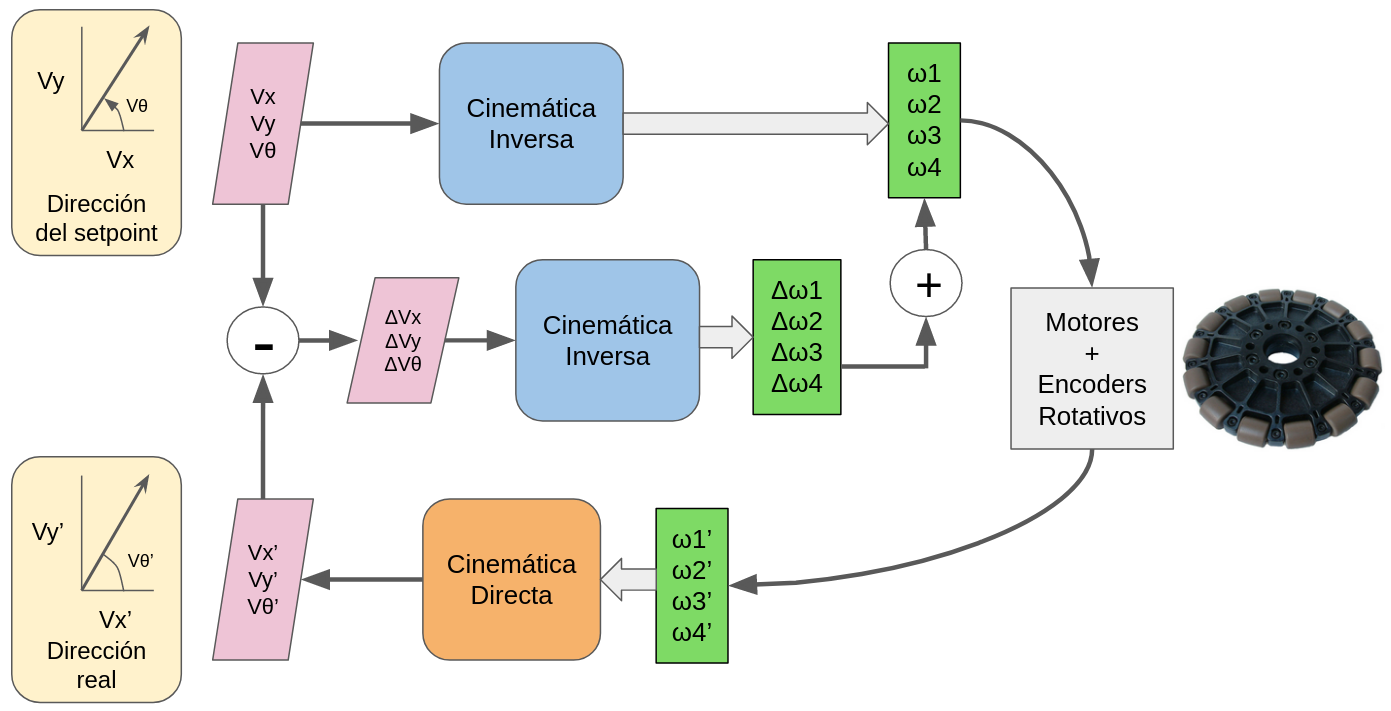
\includegraphics[width=0.9\linewidth]{images/diag_compensacion_modelo_cinem.png}
    \caption{Diagrama del Modelo Cinemático compensado}
    \label{fig:diagramamodelocinemcompensado}
\end{figure}

Los experimentos se realizaron en un entorno consistente con la iteración anterior y los resultados muestran una reducción significativa en los errores de trayectoria, demostrando la robustez del enfoque propuesto, de modo que el robot puede seguir trayectorias con desviaciones mínimas.

\paragraph{Compensación de movimiento rotacional} \mbox{} \vspace{8pt}

El enfoque propuesto es el de tener un acumulador basado en la odometría de $\theta$ que mide la distancia recorrida angularmente. El principio de funcionamiento es tal que aplica ajustes en la velocidad rotacional para compensar el desplazamiento, de modo que el robot intente llevar la distancia rotacional a cero nuevamente. Por ejemplo, si el robot detecta un desplazamiento hacia la derecha, se aumenta la velocidad rotacional hacia la izquierda para compensar el desfase en la cantidad determinada por la distancia rotacional. De este modo es posible corregir la orientación de movimiento. \\

En la Figura \ref{fig:diagsecuenciamodcinemcompens} se muestra un diagrama de secuencia sobre la implementación de la compensación del Modelo Cinemático.

\begin{figure}[htb]
    \centering
    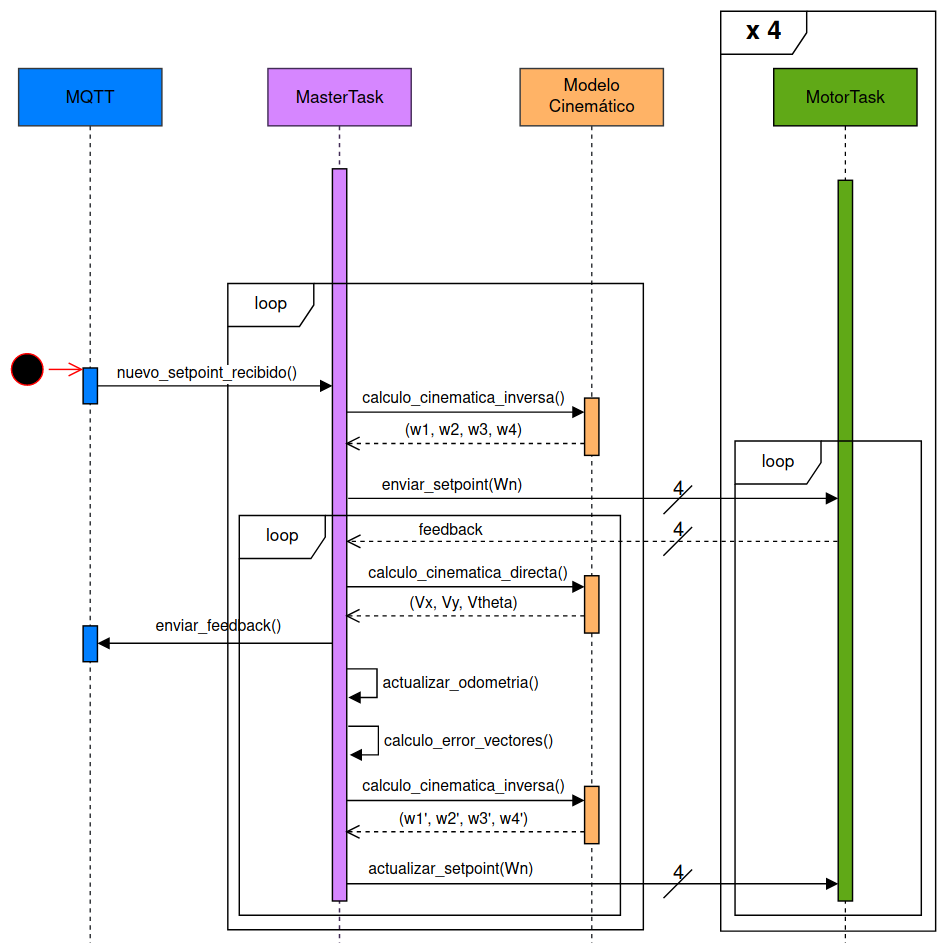
\includegraphics[width=1\linewidth]{images/diag_secuencia_modelo_cinematico_compensado.png}
    \caption{Diagrama de secuencia del Modelo Cinemático compensado}
    \label{fig:diagsecuenciamodcinemcompens}
\end{figure}


